% !TeX root=../journalDeepMedic.tex


%%%%%%%%%%%%%%%%%%%%%%%%%%%%%%%%%%%%%%%%%%%%%%%%%%%%%%%%%%%%%%
%%%%%%%%%%%%%%%%%%%% DISCUSSION %%%%%%%%%%%%%%%%%%%%%%%%%%%%%%
%%%%%%%%%%%%%%%%%%%%%%%%%%%%%%%%%%%%%%%%%%%%%%%%%%%%%%%%%%%%%%

\section{Discussion and Conclusion}
\label{sec:discussion}



We have presented DeepMedic, a 3D CNN architecture for automatic lesion segmentation that surpasses state-of-the-art on challenging data. The proposed novel training scheme is not only computationally efficient but also offers an adaptive way of partially alleviating the inherent class-imbalance of segmentation problems. We analyzed the benefits of using small convolutional kernels in 3D CNNs, which allowed us to develop a deeper and thus more discriminative network, without increasing the computational cost and number of trainable parameters. We discussed the challenges of training deep neural networks and the adopted solutions from the latest advances in deep learning. Furthermore, we proposed an efficient solution for processing large image context by the use of parallel convolutional pathways for multi-scale processing, alleviating one of the main computational limitations of previous 3D CNNs. Finally, we presented the first application of a 3D fully connected CRF on medical data, employed as a post-processing step to refine the network's output, a method that has also been shown promising for processing 2D natural images (\cite{chen2014semantic}). The design of the proposed system is well suited for processing medical volumes thanks to its generic 3D nature. The capabilities of DeepMedic and the employed CRF for capturing 3D patterns exceed those of 2D networks and locally connected random fields, models that have been commonly used in previous work. At the same time, our system is very efficient at inference time, which allows its adoption in a variety of research and clinical settings.

The generic nature of our system allows its straightforward application for different lesion segmentation tasks without major adaptations. To the best of our knowledge, our system achieved the highest reported accuracy on a cohort of patients with severe TBI. As a comparison, we improved over the reported performance of the pipeline in \cite{Rao2014b}. Important to note is that the latter work focused only on segmentation of contusions, while our system has been shown capable of segmenting even small and diffused pathologies. Additionally, our pipeline achieved state-of-the-art performance on both public benchmarks of brain tumors (BRATS 2015) and stroke lesions (SISS ISLES 2015). We believe performance can be further improved with task- and data-specific adjustments, for instance in the pre-processing, but our results show the potential of this generically designed segmentation system.

When applying our pipeline to new tasks, a laborious process is the reconfiguration of the CRF. The model improved our system's performance with statistical significance in all investigated tasks, most profoundly when the performance of the underlying classifier degrades, proving its flexibility and robustness. Finding optimal parameters for each task, however, can be challenging. This became most obvious on the task of multi-class tumor segmentation. Because the tumor's substructures vary significantly in appearance, finding a global set of parameters that yields improvements on all classes proved difficult. Instead, we applied the CRF in a binary fashion. This CRF model can be configured with a separate set of parameters for each class. However the larger parameter space would complicate its configuration further. Recent work from \cite{Zheng2015} showed that this particular CRF can be casted as a neural network and its parameters can be learned with regular gradient descent. Training it in an end-to-end fashion on top of a neural network would alleviate the discussed problems. This will be explored as part of future work.


\begin{figure}[!h]
\vspace{-20pt}
\centering
\begin{subfigure}[b]{0.95\textwidth}
	\centering
	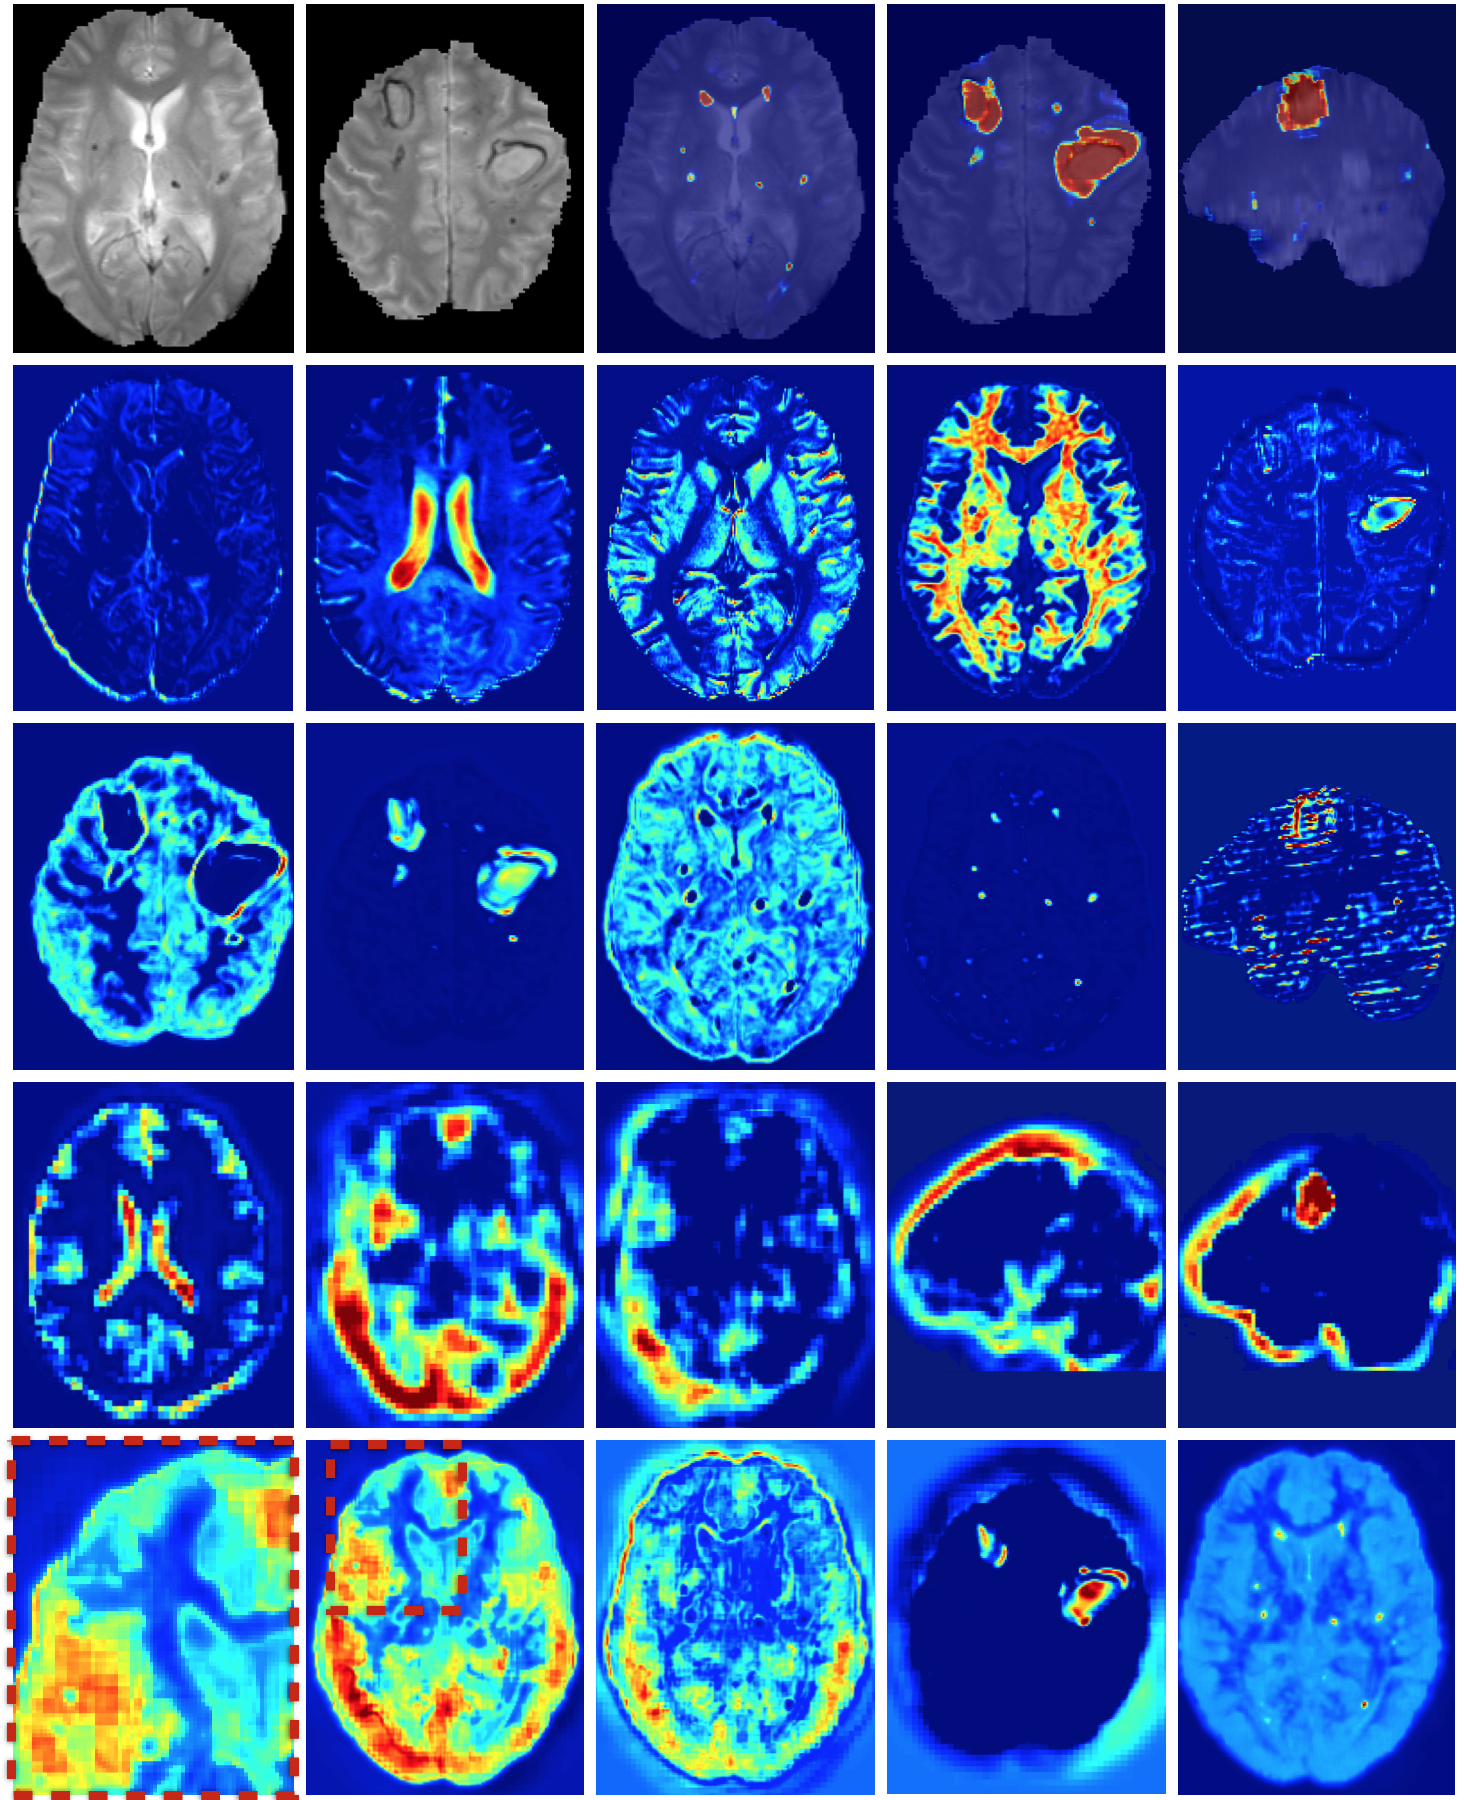
\includegraphics[clip=true, trim=0pt 0pt 0pt 0pt, width=1.0\textwidth]{figures/discussion/featureMapsFigure.png}
\end{subfigure}
\vspace{-5pt} %takes away some white space before the caption
\caption{(First row) GE scan and DeepMedic's segmentation. (Second row) FMs of earlier and (third row) deeper layers of the first convolutional pathway. (Fourth row) Features learnt in the low-resolution pathway. (Last row) FMs of the two last hidden layers, which combine multi-resolution features towards the final segmentation.}
\label{fig:featureMaps}
\end{figure}
%\vspace{-1pt} %takes away some white space after figure

The discriminative power of the learned features is indicated by the success of recent CNN-based systems in matching human performance in domains where it was previously considered too ambitious (\cite{he2015delving, Silver2016}). Analysis of the automatically extracted information could potentially provide novel insights and facilitate research on pathologies for which little prior knowledge is currently available. In an attempt to illustrate this, we explore what patterns have been learned automatically for the lesion segmentation tasks. We visualize the activations of DeepMedic's FMs when processing a subject from our TBI database. Many appearing patterns are difficult to interpret, especially in deeper layers. In Fig.~\ref{fig:featureMaps} we provide some examples that have an intuitive explanation. One of the most interesting findings is that the network learns to identify the ventricles, CSF, white and gray matter. This reveals that differentiation of tissue type is beneficial for lesion segmentation. This is in line with findings in the literature, where segmentation performance of traditional classifiers was significantly improved by incorporation of tissue priors (\cite{Leemput1999, Zikic2012}). It is intuitive that different types of lesions affect different parts of the brain depending on the underlying mechanisms of the pathology. A rigorous analysis of spatial cues extracted by the network may reveal correlations that are not well defined yet.

Similarly intriguing is the information extracted in the low-resolution pathway. As they process greater context, these neurons gain additional localization capabilities. The activations of certain FMs form fields in the surrounding areas of the brain. These patterns are preserved in the deepest hidden layers, which indicates they are beneficial for the final segmentation (see two last rows of Fig.~\ref{fig:featureMaps}). We believe these cues provide a spatial bias to the system, for instance that large TBI contusions tend to occur towards the front and sides of the brain (see Fig.~\ref{fig:spatialMap}). Furthermore, the interaction of the multi-resolution features can be observed in FMs of the hidden layer that follows the concatenation of the pathways. The network learns to weight the output of the two pathways, preserving low resolution in certain parts and show fine details in others (bottom row of Fig.~\ref{fig:featureMaps}, first three FMs). Our assumption is that the low-resolution pathway provides a rough localization of large pathologies and brain areas that are challenging to segment, which reserves the rest of the network's capacity for learning detailed patterns associated with the detection of smaller lesions, fine structures and ambiguous areas.

The findings of the above exploration lead us to believe that great potential lies into fusing the discriminative power of the \quot{deep black box} with the knowledge acquired over years of targeted biomedical research. Clinical knowledge is available for certain pathologies, such as spatial priors for white matter lesions. Previously engineered models have been proven effective in tackling fundamental imaging problems, such as brain extraction, tissue segmentation and bias field correction. We show that a network is capable of automatically extracting some of this information. It would be interesting, however, to investigate structured ways for incorporating such existing information as priors into the network's feature space, which should simplify the optimization problem while letting a specialist guide the network towards an optimal solution.

Although neural networks seem promising for medical image analysis, making the inference process more interpretable is required. This would allow understanding when the network fails, an important aspect in biomedical applications. Although the output is bounded in the $[0,1]$ range and commonly referred to as probability for convenience, it is not a true probability in a Bayesian sense. Research towards Bayesian networks aims to alleviate this limitation. An example is the recent work of \cite{Gal2015} who show that model confidence can be estimated via sampling the dropout mask.

A general point should be made about the performance drop observed when our system is applied on test datasets of BRATS and ISLES in comparison to its cross-validated performance on the training data. In both cases, subsets of the test images were acquired in clinical centers different from the ones of training datasets. Differences in scanner type and acquisition protocols have significant impact on the appearance of the images. The issue of multi-center data heterogeneity is considered a major bottleneck for enabling large-scale imaging studies. This is not specific to our approach, but a general problem in medical image analysis. One possible way of making the CNN invariant to the data heterogeneity is to learn a generative model for the data acquisition process, and use this model in the data augmentation step. This is a direction we explore as part of future work.

In order to facilitate further research in this area and to provide a baseline for future evaluations, we make the source code of the entire system publicly available.
